%=============================================================
% Header, Cover, and Preamble
%=============================================================
\documentclass[a4paper, 12pt, english]{book}
%=============================================================
\usepackage{amsmath} %use package here for formulas, maybe needed
\usepackage{graphicx} % This for Images
\usepackage{babel}
\usepackage{makeidx}
\usepackage{index}
\usepackage{datetime}
\usepackage{erewhon}
\usepackage{lipsum}
\usepackage{lettrine}
\usepackage{GoudyIn}
%\usepackage{dirtytalk}
\usepackage{color}
\usepackage{hyperref}
\usepackage[x11names]{xcolor} 
\usepackage{subcaption}
\usepackage{indentfirst}
\usepackage{enumitem,amssymb}
\usepackage{listings}
\usepackage{tikz}
\usepackage{tikz-qtree}
\usetikzlibrary{trees}
\usepackage[a4paper, inner=1.7cm, outer=2.7cm, top=2cm, bottom=2cm]{geometry}
%==============================================
\newlist{todolist}{itemize}{2}
\setlist[todolist]{label=$\square$}
\usepackage{pifont}
\newcommand{\cmark}{\ding{51}}%
\newcommand{\xmark}{\ding{55}}%
\newcommand{\done}{\rlap{$\square$}{\raisebox{2pt}{\large\hspace{1pt}\cmark}}%
\hspace{-2.5pt}}
\newcommand{\wontfix}{\rlap{$\square$}{\large\hspace{1pt}\xmark}}
%=============================================================
\hypersetup{
    colorlinks=true,
    linkcolor=black,
    urlcolor=red,
    linktoc=all
}

%>>>>>>> dev
%=============================================================
\renewcommand{\LettrineFontHook}{\color{VioletRed4}\GoudyInfamily{}}
\LettrineTextFont{\itshape}
\setcounter{DefaultLines}{3}%
%=============================================================
\makeindex
%=============================================================
\title{\textbf{Software Engineering Project Report}}
%-------------------------------------------------------------
\newdateformat{monthdayyeardate}{
	\monthname[\THEMONTH]~\THEDAY, \THEYEAR}
%=============================================================
% Beginning of The Document
%=============================================================
\begin{document}
\author{Belal Hmedan \& Deng Jianning\\University of Burgundy}
%=============================================================
\maketitle
%=============================================================
\let\cleardoublepage\clearpage
%=============================================================
\tableofcontents
%=============================================================
% The Core of Report
%=============================================================
\chapter*{Introduction}
\addcontentsline{toc}{chapter}{Introduction} \markboth{INTRODUCTION}{}
%<<<<<<< HEAD
%\lettrine{B}{uilding} an Offline Map Software is a challenging project, because it requires a good knowledge in Geography, Mathematics, Graph Theory, and Computer Science.
%\\At the very beginning of such project many questions must be asked, such as: \\Which places should the Map covers? For which application the Map will be used?
%Which Information is necessary, and Which Information is useless so it can be \\Filtered, so total amount of Data will be reduced.
%\\This Project is a try to answer some of many questions that any computer science Student will ask while starting this kind of projects. Maybe we didn't answer all The questions because of time limit, but we hope that this project will be useful For Other students to get some answers , and to get the fastest way between two Locations, That's why we selected 20 Locations carefully to satisfy the daily needs Of Students like Universities, Cool Restaurant, Pharmacy, Hospital, Shopping Centers, Students Residences, etc.
%\\This project with all cool features and nice looking objects, is nothing more than "Hello Map", because Cartography is a great science developing everyday for both Civil and military use, and everyday there is changes on our planet leads to changes On the Map, starting from Environmental changes, and not ending by Human-Made changes. 
%===============================================================
\lettrine{B}{uilding} an Offline map software is a challenging project, 
because it requires a good knowledge in Geography, Mathematics, 
Graph Theory, and Computer Science.\\

At the very beginning of such project many questions must be asked, such as: 
What places should the map covers? For which application the map will be used?
Which Information is necessary, and which information is useless so it can be 
filtered, so total amount of Data will be reduced.\\

This Project is a try to answer some of many questions that any computer 
science student will ask while starting such kind of projects. Maybe we 
didn't answer all The questions because of time limit, but we hope that 
this project will be useful For Other students to get some answers , and 
to get the fastest way between two Locations, That's why we selected 20 
locations carefully to satisfy the daily needs Of students like universities, 
cool restaurants, pharmacy, hospital, shopping centers, students residences, etc.\\

This project with all cool features and nice looking objects, is nothing more 
than "Hello Map", because Cartography is a great science developing everyday 
for both civil and military use, and everyday there is changes on our planet 
leads to remarkable changes on the Map, starting from environmental changes, and not ending by Human-Made changes. 
%>>>>>>> dev

%=============================================================
\chapter{Project Description}
%=============================================================
%<<<<<<< HEAD
\section{Goal of the Project}
The goal of this project is to develop a software to locate (and rate) various buildings, such as schools, university buildings, major offices, hospitals, various shops, cool restaurants, streets, roads, parks, and other interesting points in Le-Creusot.
The key idea is to develop a software to visualize Le-Creusot, its streets, some
buildings, roads, and parks, in which the user can perform several actions, such as asking for an itinerary between two (or passing through more) points.
%=============================================================
\section{Completeness of the Project}
%-------------------------------------------------------------
\subsection{Place Locating}
Twenty locations were provided on this project, and there is ability to add many other places due to requirements, but user can't add places, only programmer.
User's privilege on this stage of the project is limited to chose only from a list of those twenty places.
%-------------------------------------------------------------
\subsection{Place Rating}
This Feature isn't added yet, but it maybe available in next releases.
%-------------------------------------------------------------
\subsection{Routing}
Routing in this stage only by foot, expanding travel Methods to car, bicycle, and Train is possible in the following releases. 
%=============================================================
%\section{Dependencies}
%Apart from STL, I’m using Boost Graph Library (BGL), which in turn depends on other Boost libraries, which in turn depends on other Boost libraries, so I included the whole Boost libraries at once.
%\section{Data Sets Introduction}
%=============================================================
\section{Overview of the Project}

% \begin{enumerate}
% 	\item The first item
% 	\item The second item
% 	\item The third etc 
% \end{enumerate}

The goal of this project is to develop a software to show the whole picture of Le Creusot city. Apart from that, it also locates various amenities, such as schools, university buildings, major offices, hospitals, various shops, cool restaurants, streets, roads, parks, and other interesting points in Le-Creusot. With this map, user can search, rate and comment for the places of interests and do routing to get there. I the follow section, a more clear picture of the goals and achievements of this picture will be shown. \\

This project would be a great opportunity for us to practice and get a little bit more familiar with the C++. Besides, it's also a chance for us to project management. This two parts of contents will also be explain in the following.



\section{Dataset Introduction}

In this project, we decide to use OSM(open-street-map) data as the base data. OSM data provides huge amount of detailed but abstract details for users. We choose this data-set because the following advantages:

\begin{enumerate}
	\item It provide detailed data base on nodes, ways and relations. Which will be more convenient to implement the Dijkstra's algorithms for routing.
	\item With the standard format of database, this application can be applicable for other cities or even countries out of box.
	\item It is a little bit more complicated, which will help us get more practice.
\end{enumerate}

Of course, choosing this way to develop the application means more complexity, more time consuming and more difficult to manage the project. But we still go for it because no pay no gain :D

%=============================================================
\section{Completeness of the Project}
%-------------------------------------------------------------
% \subsection{Place Locating}

For this release of the application

\begin{enumerate}
	\item File I/O
		\begin{todolist}
			\item[\done] Loaded by the user
			\item[\wontfix] Modified and saved by the user
		\end{todolist}
	\item Map Displaying
	\begin{todolist}
		\item[\done] Graphically display the map 
	\end{todolist}
	\item Available Location
	\begin{todolist}
		\item[\done] Locations required in the reference is available
		\item[\done] Almost all locations contained in OSM data is available
	\end{todolist}
	\item Roads and routing 
	\begin{todolist}
		\item[\done] Presenting roads
		\item[\done] Different kinds of roads are distinguished graphically.
		\item[\done] Basic routing with 20 places as beginning or end
		\item[\wontfix] Different travel mode
	\end{todolist}
	\item Offline
	\begin{todolist}
		\item[\done] All the features is based on offline OSM data
	\end{todolist}
\end{enumerate}

% % Twenty locations were provided on this project, and there is ability to add many other places due to requirements, but user can't add places, only programmer.
% % User's privilege on this stage of the project is limited to chose only from a list of those twenty places.
% % Deng can say something here.
% %-------------------------------------------------------------
% \subsection{Place Rating}
% This Feature isn't added yet, but it maybe available in next releases.
% %-------------------------------------------------------------
% \subsection{Routing}
% Routing in this stage only by foot, expanding travel Methods to car, bicycle, and Train is possible in the following releases. 
% %=============================================================




\section{Dependencies}

\begin{enumerate}
	\item {\textbf{Boost}}\\
	Need to be installed if you don't have it. Follow the installation guide below.
		\begin{itemize}[noitemsep]
		\item {\textbf{Windows}} \\
		Using vcpkg from Microsoft (https://github.com/microsoft/vcpkg)
		you can install Boost libraries through command line window as following:\\
		vcpkg install boost
		\item {\textbf{Ubuntu}} \\
		If it is not pre-install in your Ubuntu, a single command 
		should help you do this (for Ubuntu 18.04):
		\begin{lstlisting}[language=bash]
$ apt-get install libboost-all-dev
		\end{lstlisting}
		\end{itemize}
	\item {\textbf{Libosmium}} \\
		This is a header-only library, no need for installation. 
		Just includ the header files in the project is OK to go.
		This is already put in the project repository.
	\item {\textbf{Protozero}} \\
		This is a header-only library, no need for installation. 
		Just includ the header files in the project is OK to go.
		This is already put in the project repository.
	\item {\textbf{Zlib}} \\
	Need to be installed if you don't have it. Follow the installation guide below.
		\begin{itemize}[noitemsep]
		\item {\textbf{Windows}} \\
    	Using vcpkg from Microsoft (https://github.com/microsoft/vcpkg)
		you can install Zlib library through command line window as following:\\
		vcpkg install zlib
		\item {\textbf{Ubuntu}} \\
		If it is not pre-install in your Ubuntu, a single command 
		should help you do this (for Ubuntu 18.04):
		\begin{lstlisting}[language=bash]
$ apt-get insatll zlib1g-dev
		\end{lstlisting}
		\end{itemize}
	\item {\textbf{Expat}}\\
	Need to be installed if you don't have it. Follow the installation guide below.
	\begin{itemize}[noitemsep]
	\item {\textbf{Windows}} \\
	Using vcpkg from Microsoft (https://github.com/microsoft/vcpkg)
		you can install Expat library through command line window as following:\\
		vcpkg install expat
	\item {\textbf{Ubuntu}} \\
	If it is not pre-install in your Ubuntu, a single command 
	should help you do this (for Ubuntu 18.04):
	\begin{lstlisting}[language=bash]
$ apt-get insatll expat
	\end{lstlisting}
	\end{itemize}
	\item {\textbf{PThread}} ( for Linux ) \\
	Use the following command to install the library
	sudo apt-get install libpthread-stubs0-dev
	\begin{lstlisting}[language=bash]
$ apt-get insatll expat
	\end{lstlisting}
	% \end{itemize}
	
\end{enumerate}

% Apart from STL, I’m using Boost Graph Library (BGL), which in turn depends on other Boost Library: Property Map, which in turn depends on other Boost Libraries, so I included the whole Boost Libraries at once.
% \section{Data Sets Introduction}







%>>>>>>> dev
%=============================================================
\chapter{Code Design and Structure}
%\section{Overview}




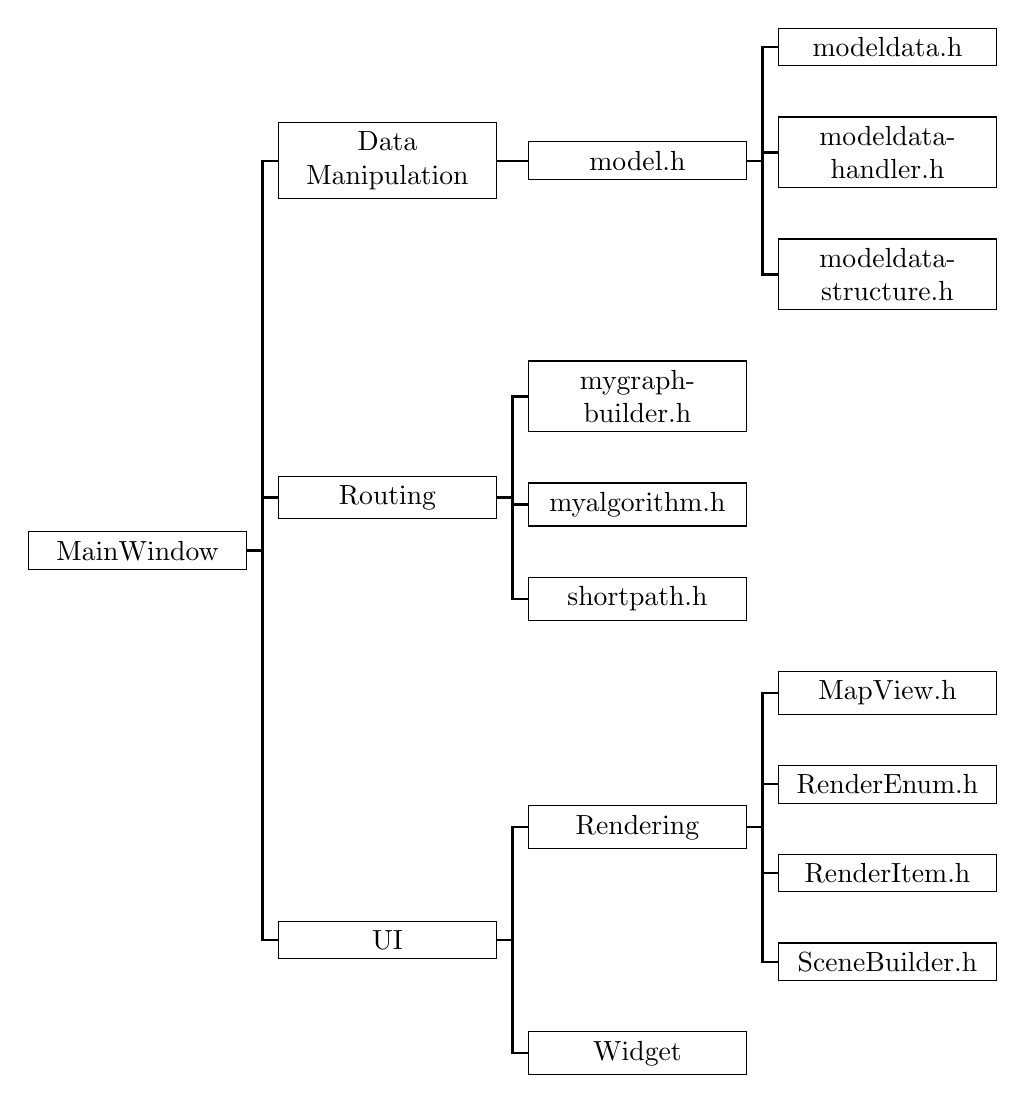
\begin{tikzpicture}[grow'=right,level distance=1.25in,sibling distance=.25in]
\tikzset{edge from parent/.style= 
	{thick, draw, edge from parent fork right},
	every tree node/.style=
	{draw,minimum width=1in,text width=1in,align=center}}
\Tree 
[. MainWindow 
	[.{Data\\Manipulation}
		[.{model.h } 
			[.{modeldata.h } ]
			[.{modeldata-\\handler.h } ]
			[.{modeldata-\\structure.h } ]
		]
	]
	[.{Routing}
		[.{mygraph-\\builder.h} ]
		[.{myalgorithm.h} ]
		[.{shortpath.h} ]
	] 
	[.{UI} 
		[.{Rendering } 
			[.{MapView.h} ]
			[.{RenderEnum.h} ]
			[.{RenderItem.h} ]
			[.{SceneBuilder.h} ]
		]
		[.{Widget } ]
	]
]
\end{tikzpicture}
\\
%=============================================================
\section{Data Manipulation}
\subsection{Overview}
This part of code aims to handle the OSM data. We use {\textit{Libosmium}} {\cite{Libosmium}} to load the file and apply basic filtering to the raw data with the code in {\textbf{modelDataHandler.h}}. That is basically a modification from the example of the library. After that, all the data will be loaded on heap using {\textit{std::map}} in the {\textbf{modelData.h}}. The file {\textbf{modelDataStructure.h}} defines the basic type of the OSM element. And {\textbf{model.h}} is the top level package of all the information we read from the file and provide interface for other part of the code to access those data. In the following subsections, I will give detailed explanations for some of those code.

\subsection{ModelData Class}

This class actually contains all available information we get from the OSM file. It is basically a container for several std::map for different kind of data( nodes, ways, relations, etc.) and other supported std::map for place searching. The reason why we load all file in the heap using map is that the interface to access data in {\textit{Libosmium}} is not so convenient. By using the std::map, we can easily access all available with the id of the data. Although it has a drawback that when we load a large file, it would takes a large mount of ram. But since we are now only focus on the city level map, this is not an issue. It also declares to friend {\textbf{modelDataHandler}} so that the OSM file data can be written in the private member of {\textbf{ModelData}}. And the handler will only be called when we load a new file, which ensures the raw data will not be modified again when the loading is finished.


\subsection{ModelDataHandler Class}

This class is modified from an example of {\textit{Libosmium}}. It is responsible for extracting data from OSM file while filtering different types of roads and buildings. This class will only be called when the user load a new file.

%=============================================================
\section{Algorithm and Routing}

This part of code organized in three different classes, each of them contains header, and source File:
%-------------------------------------------------------------
\subsection{ MyGraphBuilder Class:}
This class mainly handles data provided from our data structure represented by the Model which depends on the OSM file in its compressed format PBF.
This class mainly takes the nodes included inside ways only from the
Model as an input, then builds vertices and edges between vertices to construct the graph, which in turn will be as an input to the next stage which is nothing except Dijkstra algorithm.
The graph in my approach is \textbf{adjacency list }proposed by Boost Graph Library.
The need for this procedure comes from the fact that: finding shortest path will be implemented through an algorithm, and the algorithm deals with a graph, not a map, so I wrote this class to build the desired graph from the data structure we imported from OSM file.
The input for this class is the Model (data structure) extracted from OSM file, 
and the output is a bidirectional weighted graph.
bidirectional: because it's easy to implement, in case we want improve it to directional graph, we must do a complicated constrains, and check each tag, to see the type of transportation, and if the way was one direction, or bidirectional.
Weighted graph: because we are calculating Euclidean distance between the nodes depending on longitude, and latitude.
%-------------------------------------------------------------
\subsection{ MyAlgorithm Class:}
This class takes the graph produced on the past class MyGraphBuilder, and the source node which we will start from, and runs Dijkstra algorithm proposed by Boost Graph Library to Find the shortest path between the source node, and all other nodes in The graph.
Special function in this class called: getShortPath takes the destination node, then returns the shortest path between the source and destination only.
In case that there was no path between nodes, the path (vector) will contain only one default node, so we don't face issues due to empty vector.
%-------------------------------------------------------------
\subsection{ ShortPath Class:}
This class is just to reduce amount of code in the main window, it doesn't do much, it just takes source node, destination node, and Model, then it builds the graph from the Model using MyGraphBuilder class, and runs MyAlgorithm class, and its special function getShortPath, finally the output is our shortest path.

\subsection{Routing}
Routing on this approach is just on foot, it's possible to add more transport methods later using tag filtering, building different transport maps, vertices, and edges, but unfortunately time was short for this project !\\

Isolated nodes which doesn't belong to any way are not included in building the Graph, because our purpose is to find a way between two nodes, so I didn't build the graph with all nodes, only connected nodes which belong to way.
Euclidean distance between the nodes is our way to assign weight to edges between nodes, and of course the way or path is nothing except group of sequential edges between connected nodes.
\subsection{Difficulties during implementation:}
There is two kind of Difficulties here:
%-------------------------------------------------------------
\subsubsection{Difficulties we got rid of it:} 
%*************************************************************
\begin{enumerate}
	\item {\textbf{First difficulty was CMake didn't find some libraries:}}\\
	specially Boost Library, later we used qmake.
	\item {\textbf{Second difficulty was that edges can't be built using idType nodes:}\\
		the solution for that was mapping the idType Nodes to unsigned int indexes through a map, so each node has ID, and vertex number.}
	\item{\textbf{Third one is redundancy of nodes in different Ways:}\\
		the solution was to compare each node of way to the map we built as solution to
		problem1.2, so if the node already found, we don't add it to our map, instead we just call it and get node index.}	
\end{enumerate}
%-------------------------------------------------------------
\subsubsection{Difficulties we can solve, but it needs more time:}
%*************************************************************
\begin{enumerate}
	\item {\textbf{Supporting different travel method.}}
	\item {\textbf{Building directional graph instead of bidirectional one.}}
%	\item {\textbf{Adding reviews, and stars options to the GUI.}}
%	\item {\textbf{Adding locations on the map.}}
\end{enumerate}
%-------------------------------------------------------------
\subsubsection{Unexpected Difficulties}
Losing member of the team at critical time of the project doubled the responsibilities to do more than what we have already planned to do, and forced us to work under pressure in some parts of the project which we didn't have ideas about it before enough time.
%============================================================
\section{GUI}
%------------------------------------------------------------

\subsection{Overview}

The GUI is composed by two part of the code. One uses a class promoted from {\textbf{QGraphicsView}} for displaying the map and interact with the users. The other one is for menu bars and routing selection as a complementary interaction entry. The allowed interactions are managed by a {\textit{Finite State Machine}} in the class {\textbf{MapView}}. Those details will be well explained in the following of the report.

\subsection{Rendering}

\subsubsection{MapView Class}

This class is a class promoted from {\textbf{QGraphicsView}} which can be considered as the top level class for the rendering. It provides the users a graphical view of the map together with several ways of interactions. I decided to use the {\textbf{QGraphics}} framework because I've seen another open source rendering library {\textit{Marble}} {\cite{Marble}} with this framework. And after google a bit about this, I get to know this frame work can provide smooth graphics dealing with thousands of objects. So I decided to use it and can also get hints from {\textit{Marble}}.

\begin{figure}
	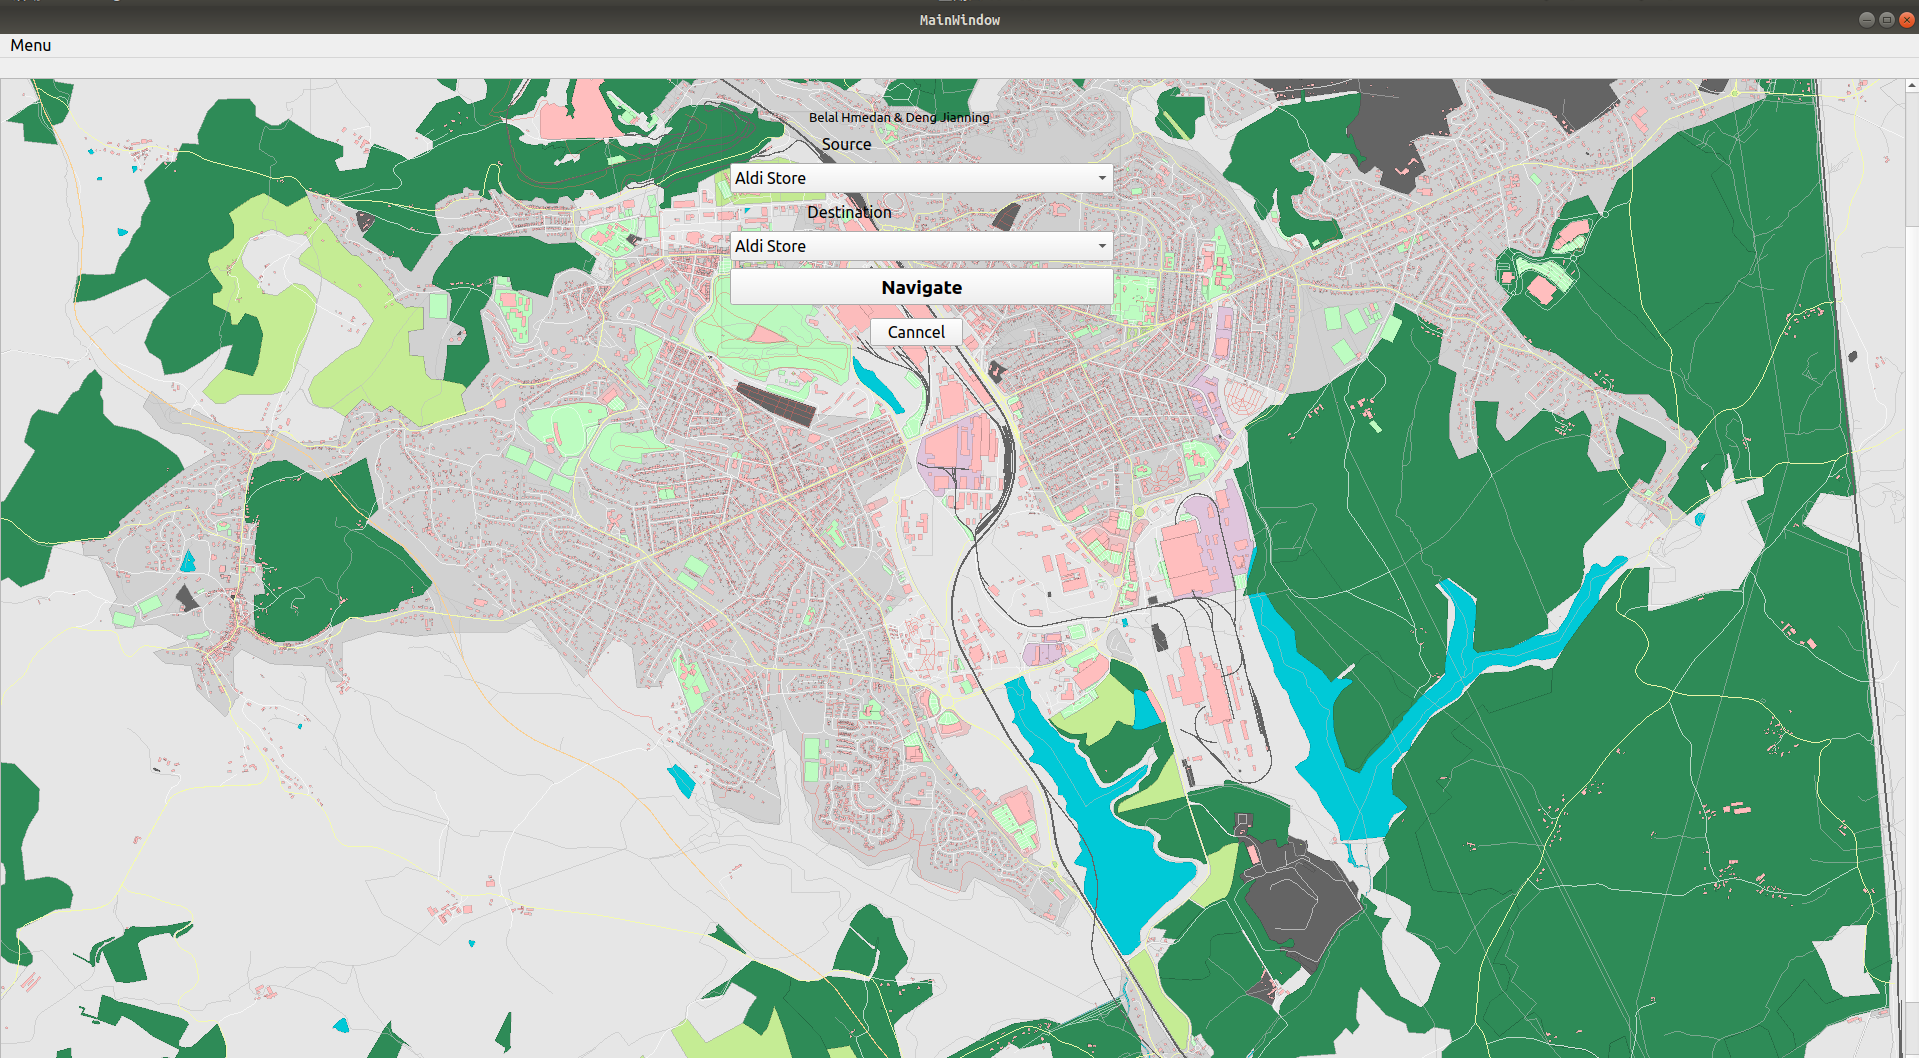
\includegraphics[width=\linewidth]{./img/rendering.png}
	\caption{Graphical View}
	\label{fig:rendering}
\end{figure}

Figure \ref{fig:rendering} shows the graphical view of a map.\\

The following functions of {\textbf{QGraphicsView}} is overridden to provide the interactions.
\begin{enumerate}
	\item {\textbf{wheelEvent(QWheelEvent *);}}
	
	This function is overridden to provide scaling of the map with mouse wheel, which is more convenient to the user. The default scaling factor is set to 0.001, ranging from 0.06 to 0.0001 with step at 1.2.	
	\item {\textbf{mousePressEvent(QMouseEvent *);}}
	
	This function enables users to drag the map and to select buildings directly on the map. At the very beginning of this design is thought as an entry for building details, ratings, comments and choosing routing places. But since we don't have time to implement the user rating system and routing algorithms will cause crashes when it failed to find a path, this entry now is hook to an empty operation with a right click menu. 
	
	\item {\textbf{contextMenuEvent(QContextMenuEvent *);}}
	
	This function will provide users an access to a right click menu, which is controlled by an embedded {\textit{finite state machine}}. The state and transition of the {\textit{finite state machine}} is explained in figure \ref{fig:FSM}.
	\begin{figure}[h!]
		\centering
		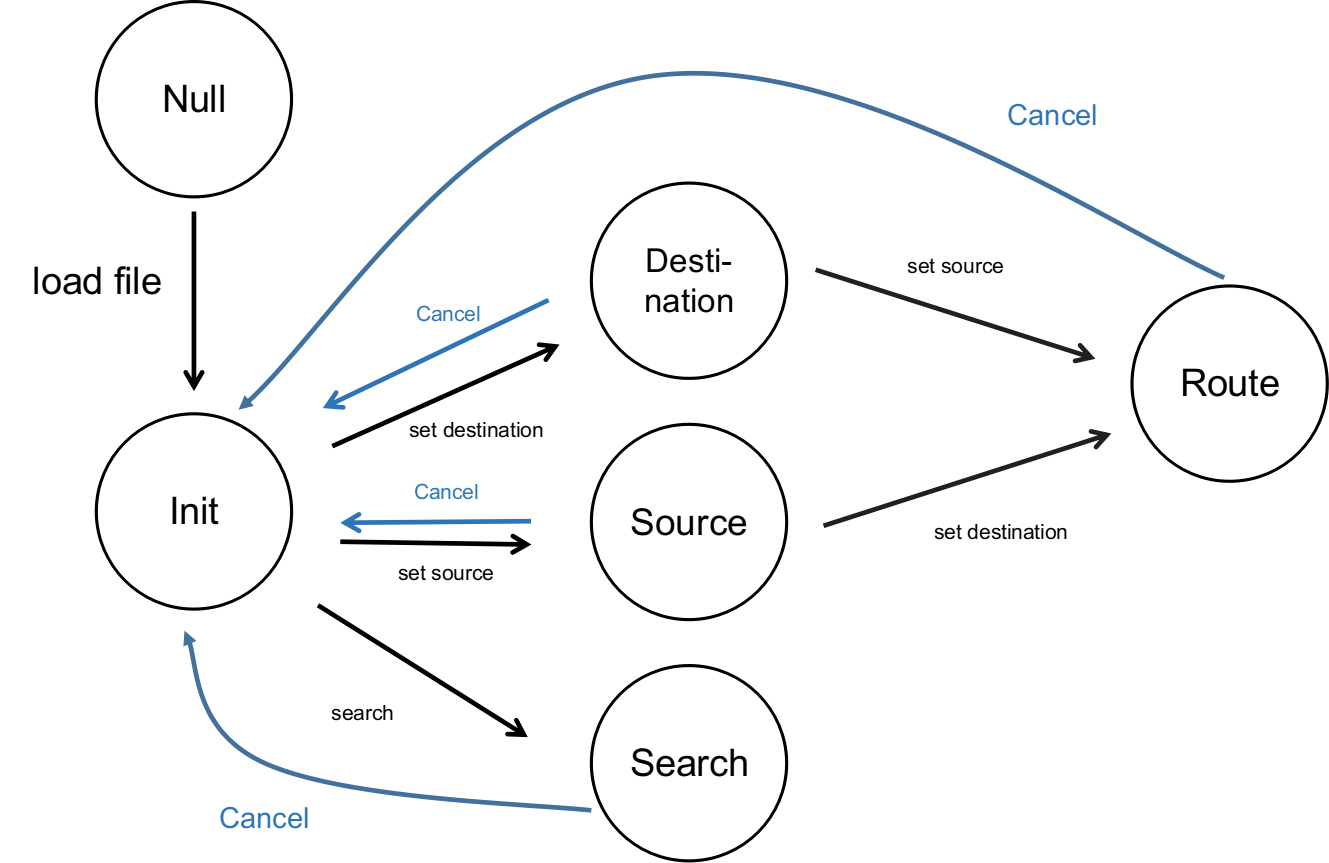
\includegraphics[width=0.7\linewidth]{./img/FSM.png}
		\caption{FSM}
		\label{fig:FSM}
	\end{figure}

	The user state was set to {\textit{Null}} before loading the data file. In this state all the interaction will be disable to avoid segmentation fault. Once the data file is loaded, the state will change to {\textit{Init}} to enable all the interactions. And the state will get changed as the user choose different options in the right click menu. And the option {\textit{cancel}} will reset the state to {\textit{Init}}. This help sort the logic for development. And the visual feedback is shown in figure \ref{fig:rightClickMenu}.
	\begin{figure}[h!]
		\centering
		\begin{subfigure}[b]{0.4\linewidth}
			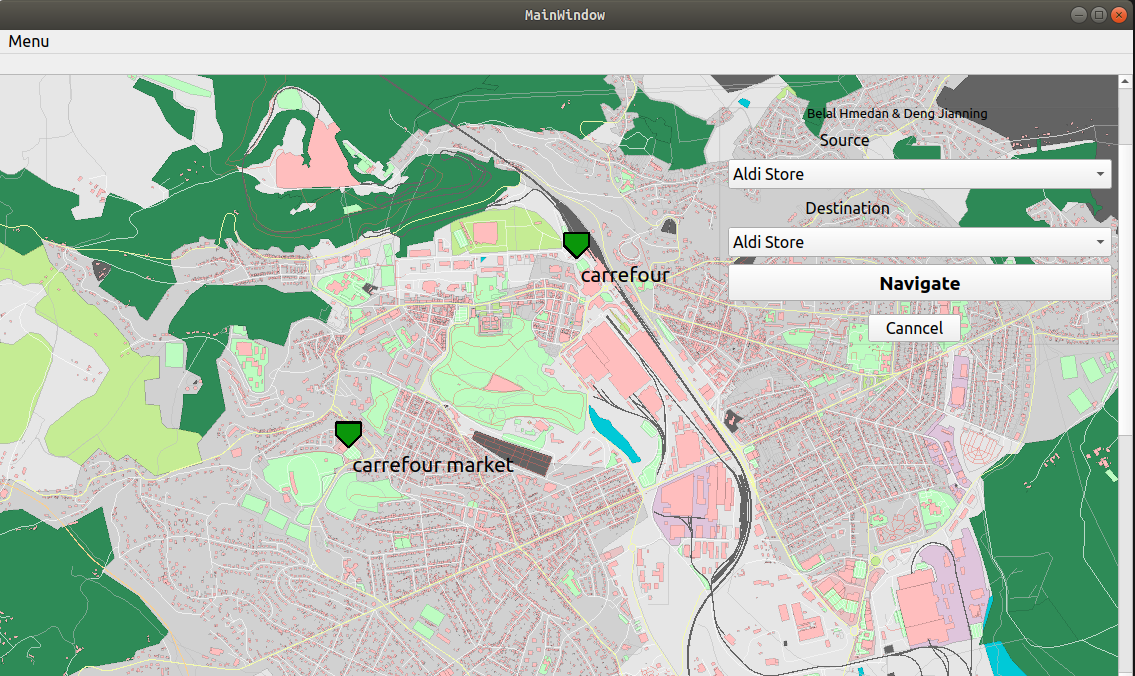
\includegraphics[width=\linewidth]{./img/search.png}
			\caption{Place Searching}
		\end{subfigure}
		\begin{subfigure}[b]{0.4\linewidth}
			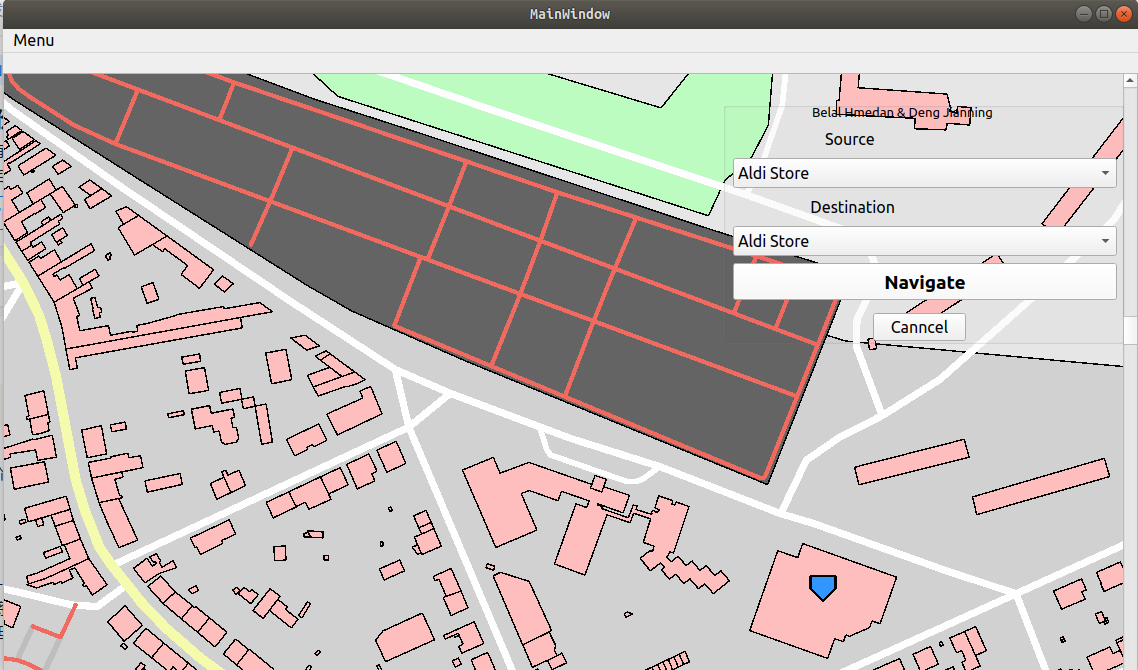
\includegraphics[width=\linewidth]{./img/selSrc.png}
			\caption{Select route source.}
		\end{subfigure}
		\begin{subfigure}[b]{0.4\linewidth}
			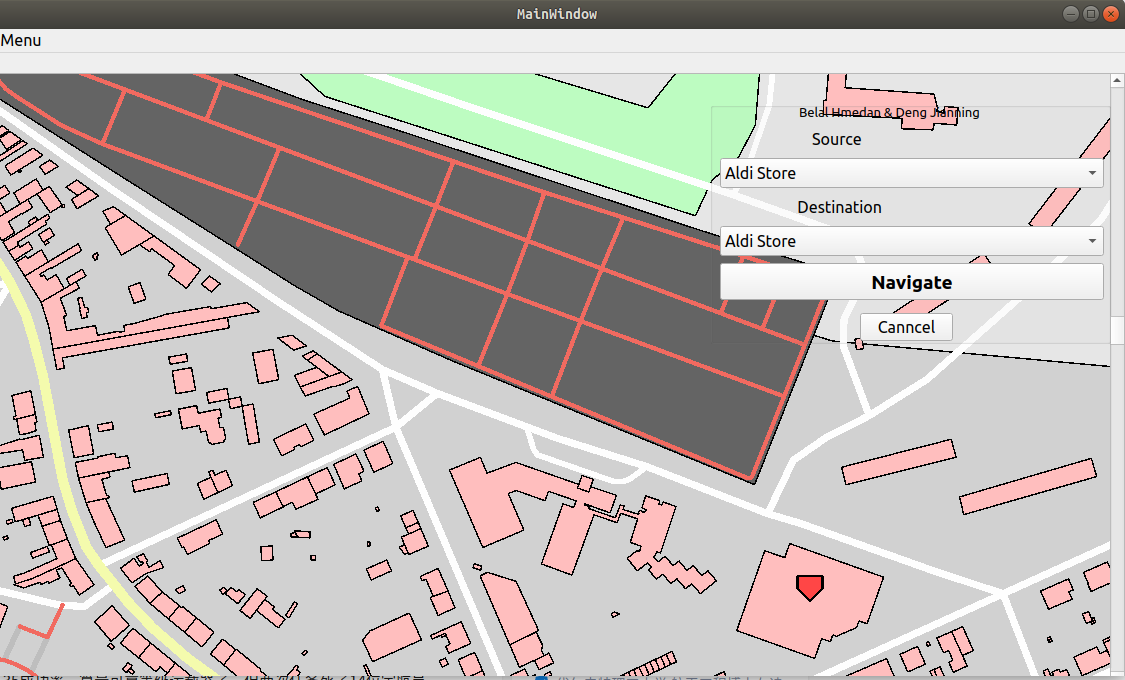
\includegraphics[width=\linewidth]{./img/selDest.png}
			\caption{Select route destination.}
		\end{subfigure}
		\caption{Visual feedback for right click menu}
		\label{fig:rightClickMenu}
	\end{figure}
	
\end{enumerate}
%\newpage
\subsubsection{SceneBuilder}

This part of code responsible for creating a proper scene for {\textbf{MapView}} to display. It also provides an interface for drawing routes and pins. This class extracts information form the {\textbf{modelData}} to form multi polygons for builds and poly lines for roads and path. 

\subsubsection{RenderItem}

This part of the code is to construct several basic item of the map rendering using {\textbf{QGrphicsItem}}. And in those items, we use enumerators to help set the z-value. The category logic uses ideas from {\textit{IO2D demo: Maps}} {\cite{IO2D}}, but not exactly the same. There're two types of enumerator for polygons and roads, which are specified in {\textbf{renderItemEnum.h}} file. Also, they are rendering styles are based on its type.

\subsection{Difficulties for rendering}

When developing this part of code, you need to have a global view of the whole project. Because this part is the bridge between database, graphical view and user interface. Which means your are dealing all the information you can get in the project. So, if we divide this part to several key points, those are the problems we solved:
\begin{enumerate}
	\item filter and categorized the proper element from OSM data for rendering
	\item properly draw buildings and roads in the {\textit{QGraphics}} framework
	\item locate the object in the view
	\item build a right click menu for users
	\item interaction logic control
	\item interface for routing algorithm
	\item visualize the place searching result and place selection
\end{enumerate}

To achieve those above requires a certain knowledge on OMS database and Qt graphical development. Since both of them are pretty new to us, we need to spend more time to read and learn. And that results in a more difficult project management. Because you just don't have enough knowledge to estimate how much time you need to spend on this.

\subsection{Widget}
Running the program that will show a window with a Menu and four buttons source, destination, navigate, and cancel.
%------------------------------------------------------------
\begin{center}
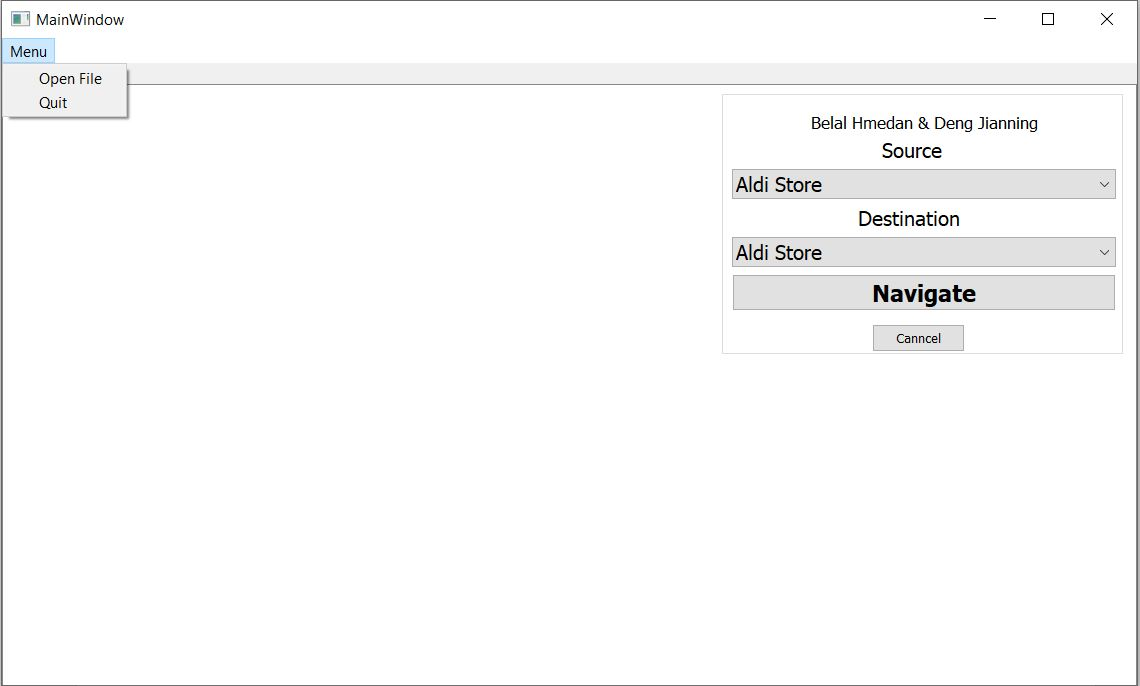
\includegraphics[width=.6\textwidth]{GUI_NoMap.JPG}
%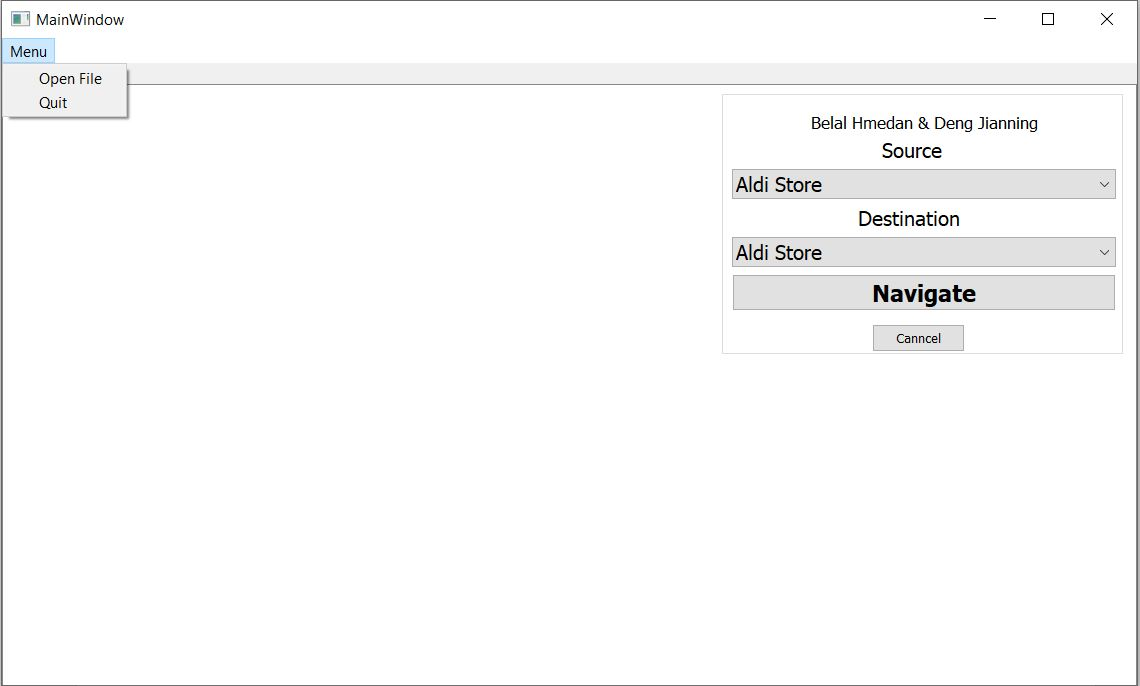
\includegraphics[width=.6\textwidth,natwidth=1200,natheight=700]{GUI_NoMap.JPG}
\end{center}
%------------------------------------------------------------
To start working, you should select (Menu - Open )
to open the map file, which should be with (.pbf) extension.
After you select your map, the software loads the map file showing the map.
%------------------------------------------------------------
\begin{center}
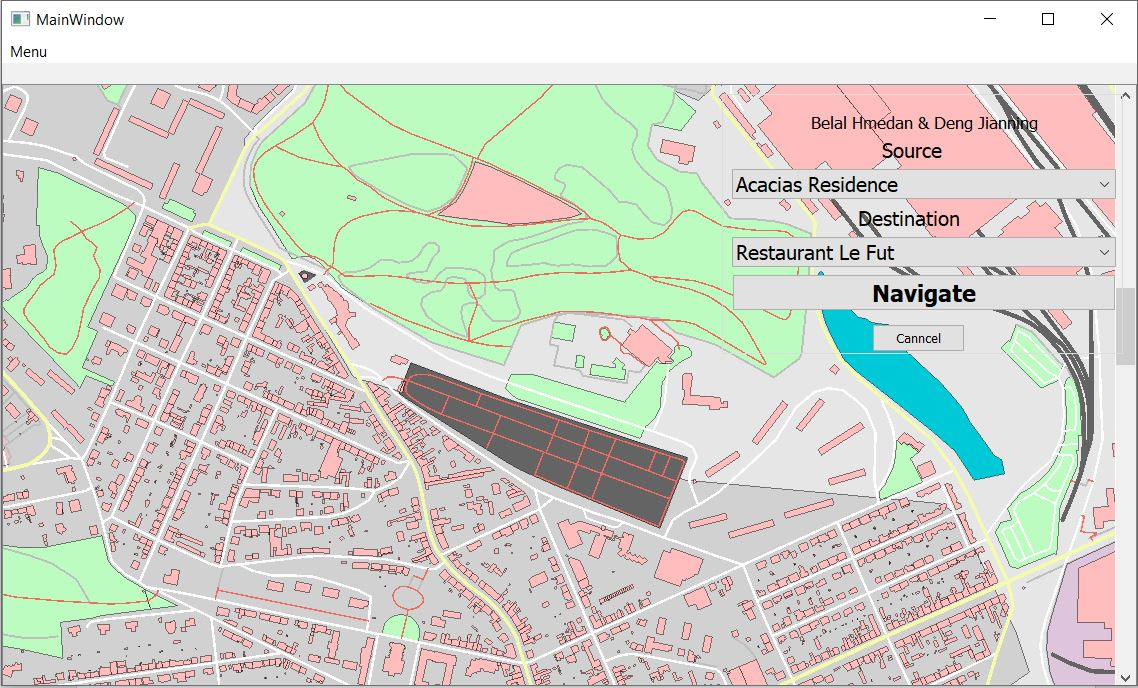
\includegraphics[width=.6\textwidth]{GUI_Map0.JPG}
%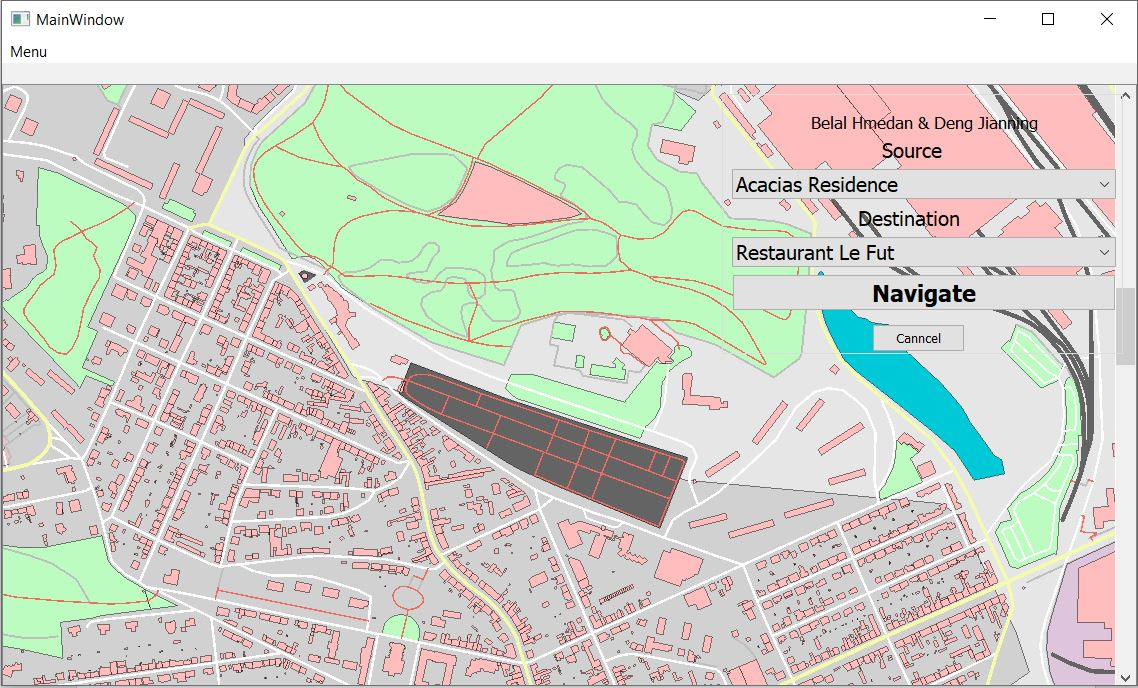
\includegraphics[width=.6\textwidth,natwidth=1200,natheight=700]{GUI_Map0.JPG}
\end{center}
%------------------------------------------------------------
The Drop-down lists source, and destination contains 20 places for each of them, all on Le Creusot city, where you can select your start point, and destination.
%------------------------------------------------------------ 
\begin{center}
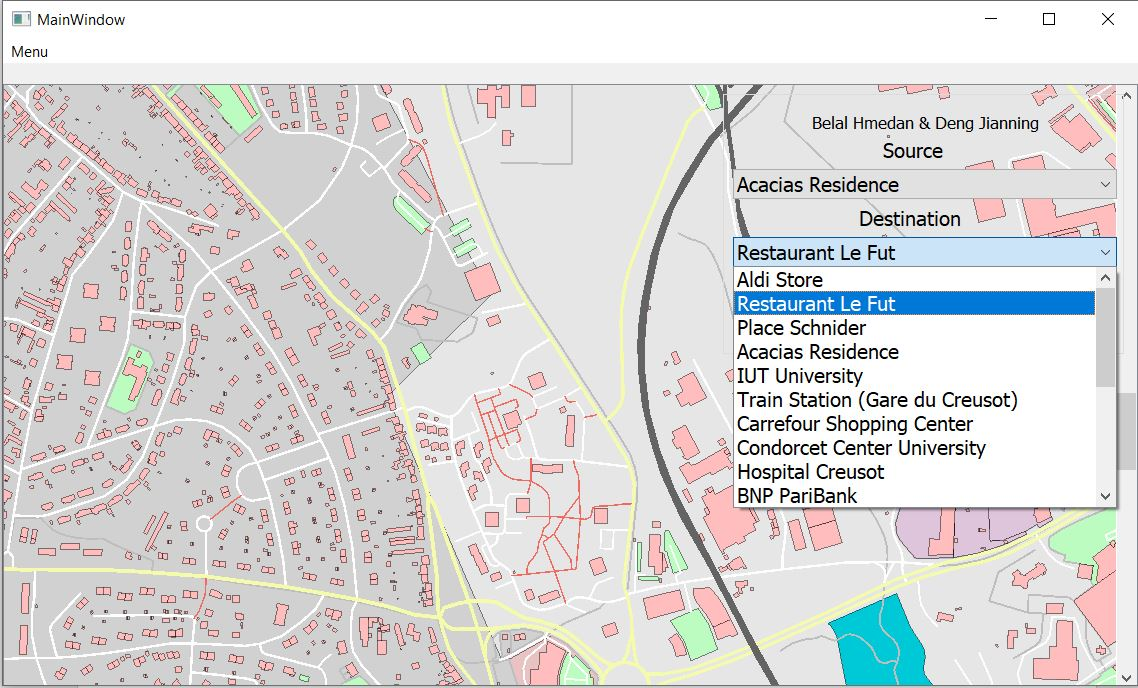
\includegraphics[width=.6\textwidth]{GUI_Map1.JPG}
%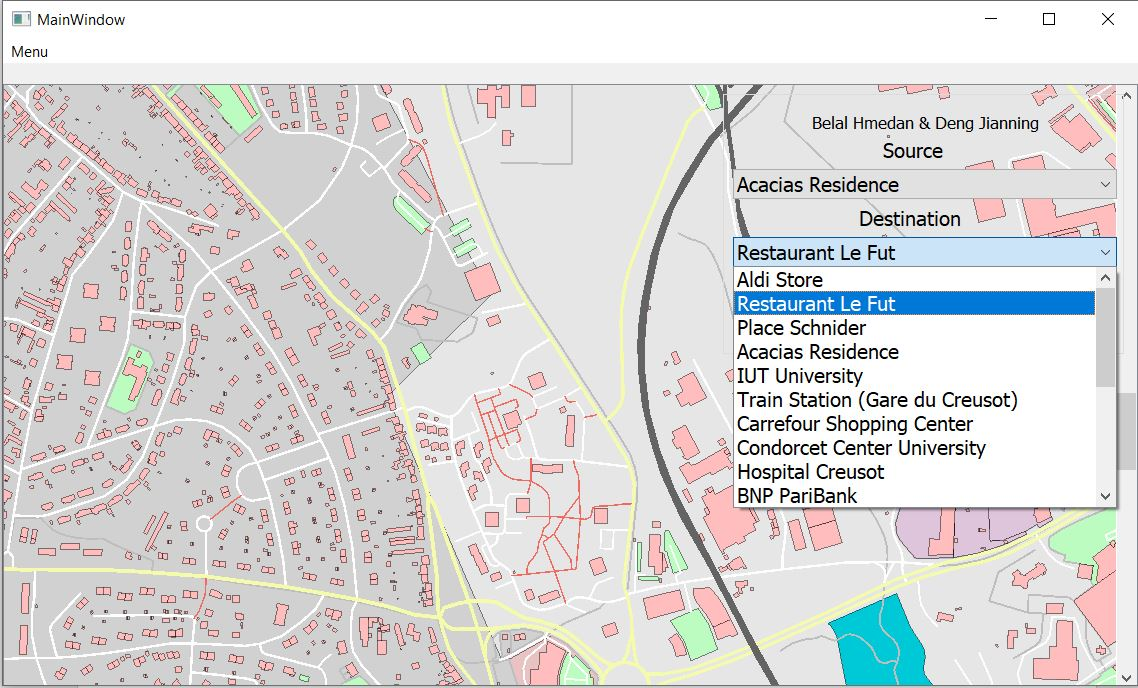
\includegraphics[width=.6\textwidth,natwidth=1200,natheight=700]{GUI_Map1.JPG}
\end{center}
%------------------------------------------------------------
by clicking on navigate button, the shortest path will be drawn by red , so you can see the way you should follow.
%------------------------------------------------------------
\begin{center}
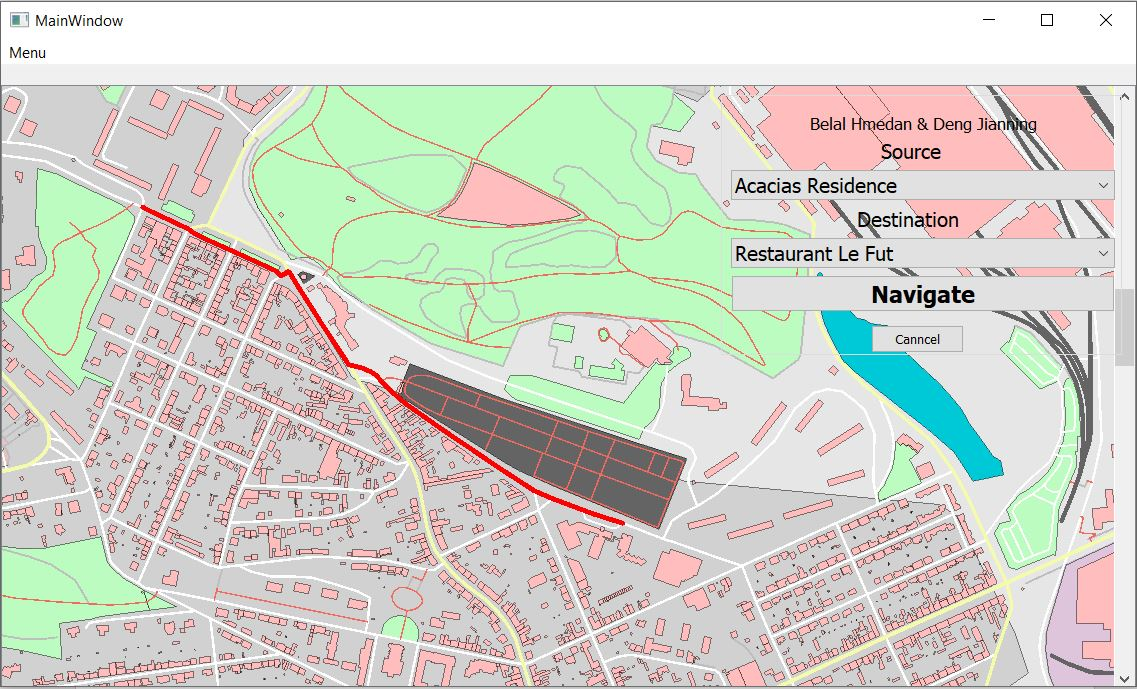
\includegraphics[width=.6\textwidth]{GUI_Map2.JPG}
%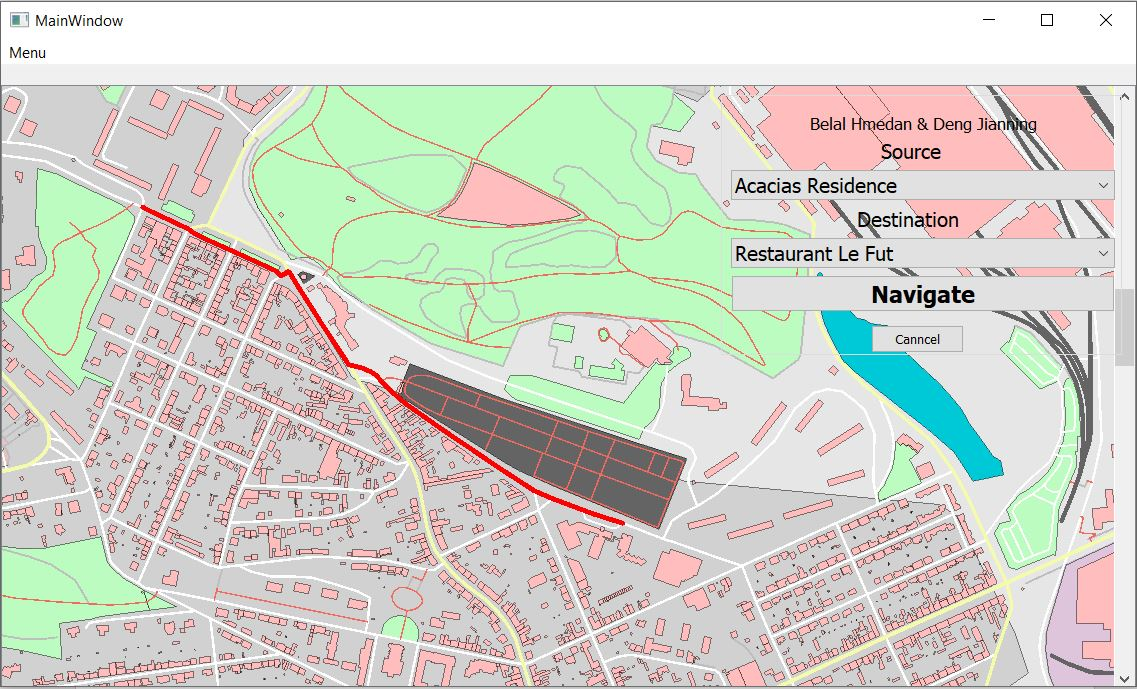
\includegraphics[width=.6\textwidth,natwidth=1200,natheight=700]{GUI_Map2.JPG}
\end{center}
%------------------------------------------------------------
Cancel button is to hide that path, and you can choose again your start point and target, so your path again will be drawn for you.
To finish, you can select (Menu - Quit) to exit the software.
%=============================================================
\subsection{Implementation ideas for comment and rating system}

Although we didn't implement the rating system, but doing this is very straight forward in our design. All we need to do is:
\begin{enumerate}
	\item A file on the file system to store the information
	\item A pop-out page when user click on the building
	The pop-out page will show detail information about this building. And in this page, we will implement a input text line or other widget for the user. Since we can retrieve the way id on the mouse click, we can store the information as a key-value pair with way id.
	\item Write the user input in the file and store them.
	Do remember to load this file when loading the map so that the information can be linked together through way id.
\end{enumerate}
%=============================================================
\chapter{Project Management}
%=============================================================
\section{Overview of the Project Planning}

We received the project at the end of September and the deadline is in Dec. 14Th. So, we have about two and a half months' time for this project. Then after we teamed up with 3 students, we decided to divided the project in 3 different periods. First is the research period. We would spend about a month's time to study about this project. After having a basic directions, we shall then move to the second period development, which will also last for about a month. And at last we plan to release the application for test, so that we can fix some bugs and prepare our documentation. All the details about the research period is logged in the discussion log of this repository. \\
At about the beginning of October, when we have a basic direction, we decided to divide this project into three main functional part: 
\begin{enumerate}
	\item {\textbf{Data Manipulation}}\\
	
	This part will handle the OSM data input, building friendly interface for rendering and routing. So, it requires an in-depth understanding on the OSM data. Apart from that, it will also help build the user rating and comment database.
	\item {\textbf{Map Rendering}}\\
	
	This part aims to render the OSM data, provide a graphical view of the map. It will also help build some common interactions like zooming, dragging and etc. Besides, it also need to provide the entry for user to rate and comment a place.
	\item {\textbf{Routing}}\\
	
	This part is trying to implement routing algorithms on the OSM data.
\end{enumerate}

So far, everything seems to be nice and neat. However, at Nov. 11Th, one of our member choose to leave the team because of the different implementation ideas. So, we need to change our plan to guarantee a basic functional version can be done on time. So, the following will be the new work assignment to the two of us.

\subsubsection{Belal}

\begin{enumerate}
	\item Routing algorithm implementation
	\item Basic GUI widget
\end{enumerate}

\subsubsection{Deng}
\begin{enumerate}
	\item Basic data manipulation(reading OSM file only)
	\item Map rendering
\end{enumerate}

With those work, we can at least purpose a functional map application. And user rating and commenting will be considered as a advanced features, which means it has the lowest priority in this project.

% We Received the Project on 30Th of September,it took us about 2 weeks to 
% team up in a group of 3 students, then we started The Research for the 
% Project since 15Th of October, Research for this project took 3 weeks 
% until 6Th of November, There was many choices, and due to strict conditions such as: the Project should work under different operating systems, we excluded promising solutions such as "Libsmscout" which was easy to use Library with advanced features, but it doesn't work on Windows, only Linux, that lead us to more complicated choices such as "Libosmium" and "Boost" Libraries.
% %>>>>>>> dev
% The Implementation started on the 6Th of November, each student worked on different part of the project: "Data Manipulation and Map Rendering" for Deng, "Shortest Path Algorithm" for Belal, and "Graphical User Interface" for Our Third Partner.
% Ten Days later At 16Th of November Deng Proposed Three Solutions for dealing with the Project:
% \begin{enumerate}
% \item {\textbf{ First solution: Using one-for-all library.}}
% \item{\textbf{Second solution: Using OSM data access library.}}
% \item{\textbf{Third solution: Display the map using Image.}}
% \end{enumerate}
% %-------------------------------------------------------------
% At that Point Belal and Deng Agreed on the second solution, because we want to propose something different and more advanced than image solution.
% Our partner preferred to go on different direction with third solution, so we had to work on the project as a team of two members only !.
% Following the advice to "Expect what is Unexpected " we reduced the project size and features so we can finish it before deadline.
% A week later, on 24Th of November we had our first working project with minimum features available, a week later on the 1st of December We did a simple GUI to deal with our map.
% Writing The Documentation took a week until 7Th of December, and writing the report in \textbf{\LaTeX} \space took another week up to 14Th of December, so We did it on time.

%-------------------------------------------------------------
%<<<<<<< HEAD
\section{Work schedules}

This section contains a detailed schedule for each member in the team.

%We divided the tasks to all team members, so every member has his own schedule of work due to his task and time.
%-------------------------------------------------------------
\subsection{Belal schedule}
%-------------------------------------------------------------
%-------------------------------------------------------------
\begin{enumerate}
\item {{\Large October\par}}
\textbf{Independent Research on, from 1st of October to 31 October}\\
%-------------------------------------------------------------
\textbf{Task (1) :} Duration 20 days.
\begin{enumerate}
\item {Get familiar with OSM data structure.}
\item {Basic Math for path planning on map:}
%*************************************************************
\begin{itemize}
    \item {Graph Theory review.}
    \item {Data Structures review.}
    \item {Algorithms review.} 
\end{itemize}
%*************************************************************
\end{enumerate}
%-------------------------------------------------------------
\textbf{Task (2) :} Duration 11 days.
\begin{enumerate}
\item {General implementation methods on map application}
%*************************************************************
\begin{itemize}
    \item{Writing The pseudo code of the algorithm}
    \item{Specifying Data Requirements :\\
              Inputs - Outputs - Data Structure to be used.}
\end{itemize}
%*************************************************************
\item {Check available libraries}

\end{enumerate}
%-------------------------------------------------------------
%-------------------------------------------------------------
\item {{\Large November\par}}
\textbf{Implementation, and Integration, from 1st of November to 30 November}\\
%-------------------------------------------------------------
\textbf{Task (1) :} Duration 22 days.
\begin{enumerate}

\item {Understanding standard templates library, boost graph library, and implementing them}
%*************************************************************
\begin{itemize}
    \item {Understanding vector and map objects.}
    \item {Understanding how to build a graph using boost graph library}
    \item {Interfacing Dijkstra algorithm from boost graph library  with the Model (data structure of the Project.\\} 
\end{itemize}
%*************************************************************
\end{enumerate}
%-------------------------------------------------------------
\textbf{Task (2) :} Duration 8 days.\\
Building friendly user interface to interact with user.

%-------------------------------------------------------------
%-------------------------------------------------------------
\item {{\Large December\par}}
\textbf{Writing documentation, report, and preparing the presentation, from 1st of December to 14 December}
\begin{enumerate}

\item {Documentation writing.}
\item {Report writing.}
\item {Preparing defense presentation.}

\end{enumerate}
%-------------------------------------------------------------

\end{enumerate}
%=============================================================
%-------------------------------------------------------------
\subsection{Deng schedule}

\subsubsection{Research Period}

	{\textbf{From Oct. 06 to Nov. 06:}} The main task in this period is to gather enough information about this project and form a big picture of it. 

\begin{enumerate}
	\item Get familiar with OSM data
	\item Research on libraries about rendering\\
	{\textit{Cartotype, Marble, IO2D, mapnik}}
	\item Read source codes in {\textit{Marble}} and {\textit{IO2D}}
	\item Read source codes and examples of {\textit{Libosmium}}
	\item Learn how to draw polygon using {\textit{QPainter}}
	\item Estimate if it is possible to build our own rendering library\\
	Documents for {\textit{Marble}} is not so detailed and the source code is too complicated for us.
	\item Think how to construct a easy-to-use database
\end{enumerate}


\subsubsection{Development Period}

	{\textbf{From Nov. 06 to Nov.17:}}

\begin{enumerate}

	\item Try to run and modified example code of {\textit{Libosmium}}
	\item Implement the basic database using C++ STL.
	\item Learn how to use {\textit{QGraphics}} framework and its interaction mechanism
	\item Try to dray simple things with {\textit{QGraphics}} framework
	\item Try to use data from database to draw buildings
	
\end{enumerate}

	{\textbf{From Nov. 17 to Nov. 30:}}
\begin{enumerate}
	\item Sort useful data from database for rendering(buildings and roads)
	\item Tweak the style and z-value for the {\textit{QGraphicsItem}}
	\item Update interface for routing
	\item Implement item retrieving for the rendering
	\item Design user interaction logic using {\textit{finite state machine}}
	\item Get familiar and implement with signal and slot for interaction
 	\item Implement place searching and visualize the result
\end{enumerate}


\subsubsection{Document Period}

{\textbf{From Dec. 01 to the deadline of this project:}}
\begin{enumerate}
	\item Fix bugs in place searching to avoid crashes\\
	Segmentation fault for those object without tag: name
	\item Fix bugs in widgets to avoid crashes\\
	Segmentation fault when clicking on the button before loading the file
	\item Fix bugs in FSM\\
	Segmentation fault because of incomplete reset to state {\textit{init}}
\end{enumerate}



%-------------------------------------------------------------


%>>>>>>> dev
%\section{Plans VS Actual}
%\say{{\Large A goal without a plan is just a wish.\par}\say{Antoine de Saint-Exupéry}}
%We started planning at earlier stage, that gave us the advantage of evaluation many solutions, and taking a look into some promising solutions, what we did over this project was not so far from what we have planned to do, but of course there is some points which we did planned to do it, but we couldn't due to time factor.
%The graphical user interface, travelling methods, and giving more choices to the user like adding a place or rating it, we hope that we can improve that in the next release so the user has the ability to do more things.

%-------------------------------------------------------------
%=============================================================
\chapter{Summary}
For this project, we worked for about two months on the design and implementation of the offline map using C++ with Qt.Throughout the project, we learned many things about Geography, Graph Theory, well-implemented coding, time management, team work, and how to use software engineering to build a project for solving real life problems.\\

In this report, we justified our approach for the problem, with all technical details, codes, and results. We presented our use of OSM dataset, Qt Graphics, Dijkstra algorithm, and finally the handy GUI integrating all theses classes together to produce our final software. We thank every tough problem that sharpened our programming and problem solving skills. Our confidence grew once we realize all we need is just more hardworking and persistence.\\

However, our output is still not perfect yet. We can recommend many modifications
to be done as future work. For example, making the graph directional instead of bidirectional, using more accurate way than Euclidean distance, and adding more traveling methods (such as train, bus, and bicycle), and adding rate and review features.


%=============================================================
\begin{thebibliography}{12}
\bibitem{Libosmium}
github: https://github.com/osmcode/libosmium
\bibitem{Marble}
website: https://marble.kde.org/index.php
\bibitem{IO2D}
website: https://kazakov.life/2018/06/07/io2d-demo-maps/
\bibitem{BGL} 
Jeremy G. Siek,
Lie-Quan Lee, Andrew Lumsdaine.
\textit{The Boost graph library : user guide and reference manual.} , ``Book," \emph{BGL}, pp. 161-322,Pearson Education, Inc., Reading, Massachusetts, 2002.
\end{thebibliography}
%=============================================================
\end{document}